%!TEX root = ../data-imputation.tex
\section{Results}
\label{sec:results}

In this section, we describe and visualize the results of our experiments.

Our goal was to provide as broad an overview as possible of the performance of various imputation methods. Therefore, we included a lage number of datasets in our selection, with different data and task types. To make the results comparable on such heterogeneous data, we decided to use the following approach.

The \textit{imputation rank} is the rank of the six imputers imputation performance on a single dataset-column combination. The values therefore lie within the interval [1, 6]. For numerical columns it is based on RMSE where lower is better. And for categorical columns it is based on the F1 macro score where higher is better. $n$ imputers with equal performance are assigned the same rank $r$ and the next best imputer gets the rank $r+n$. This is also known as \textit{standard competition ranking} ("1224" ranking). If an imputation mehtods produced Null-values we set it's rank to be the last.

Of course, this ranking simplifies the results. However, comparing the merics (F1, RMSE) across tasks/columns is not sensible. Especially for RMSE, where the values do not lie within a well-defined range.


% Experiment / Scenario / Task Type
% - observations
%   - best imputers
%   - medium imputers
%   - worst imputers
% - bottom line


\subsection{Experiment 1: Imputation Quality}


\subsubsection{Scenario 1: Training on Complete Data}


\begin{figure}\centering
    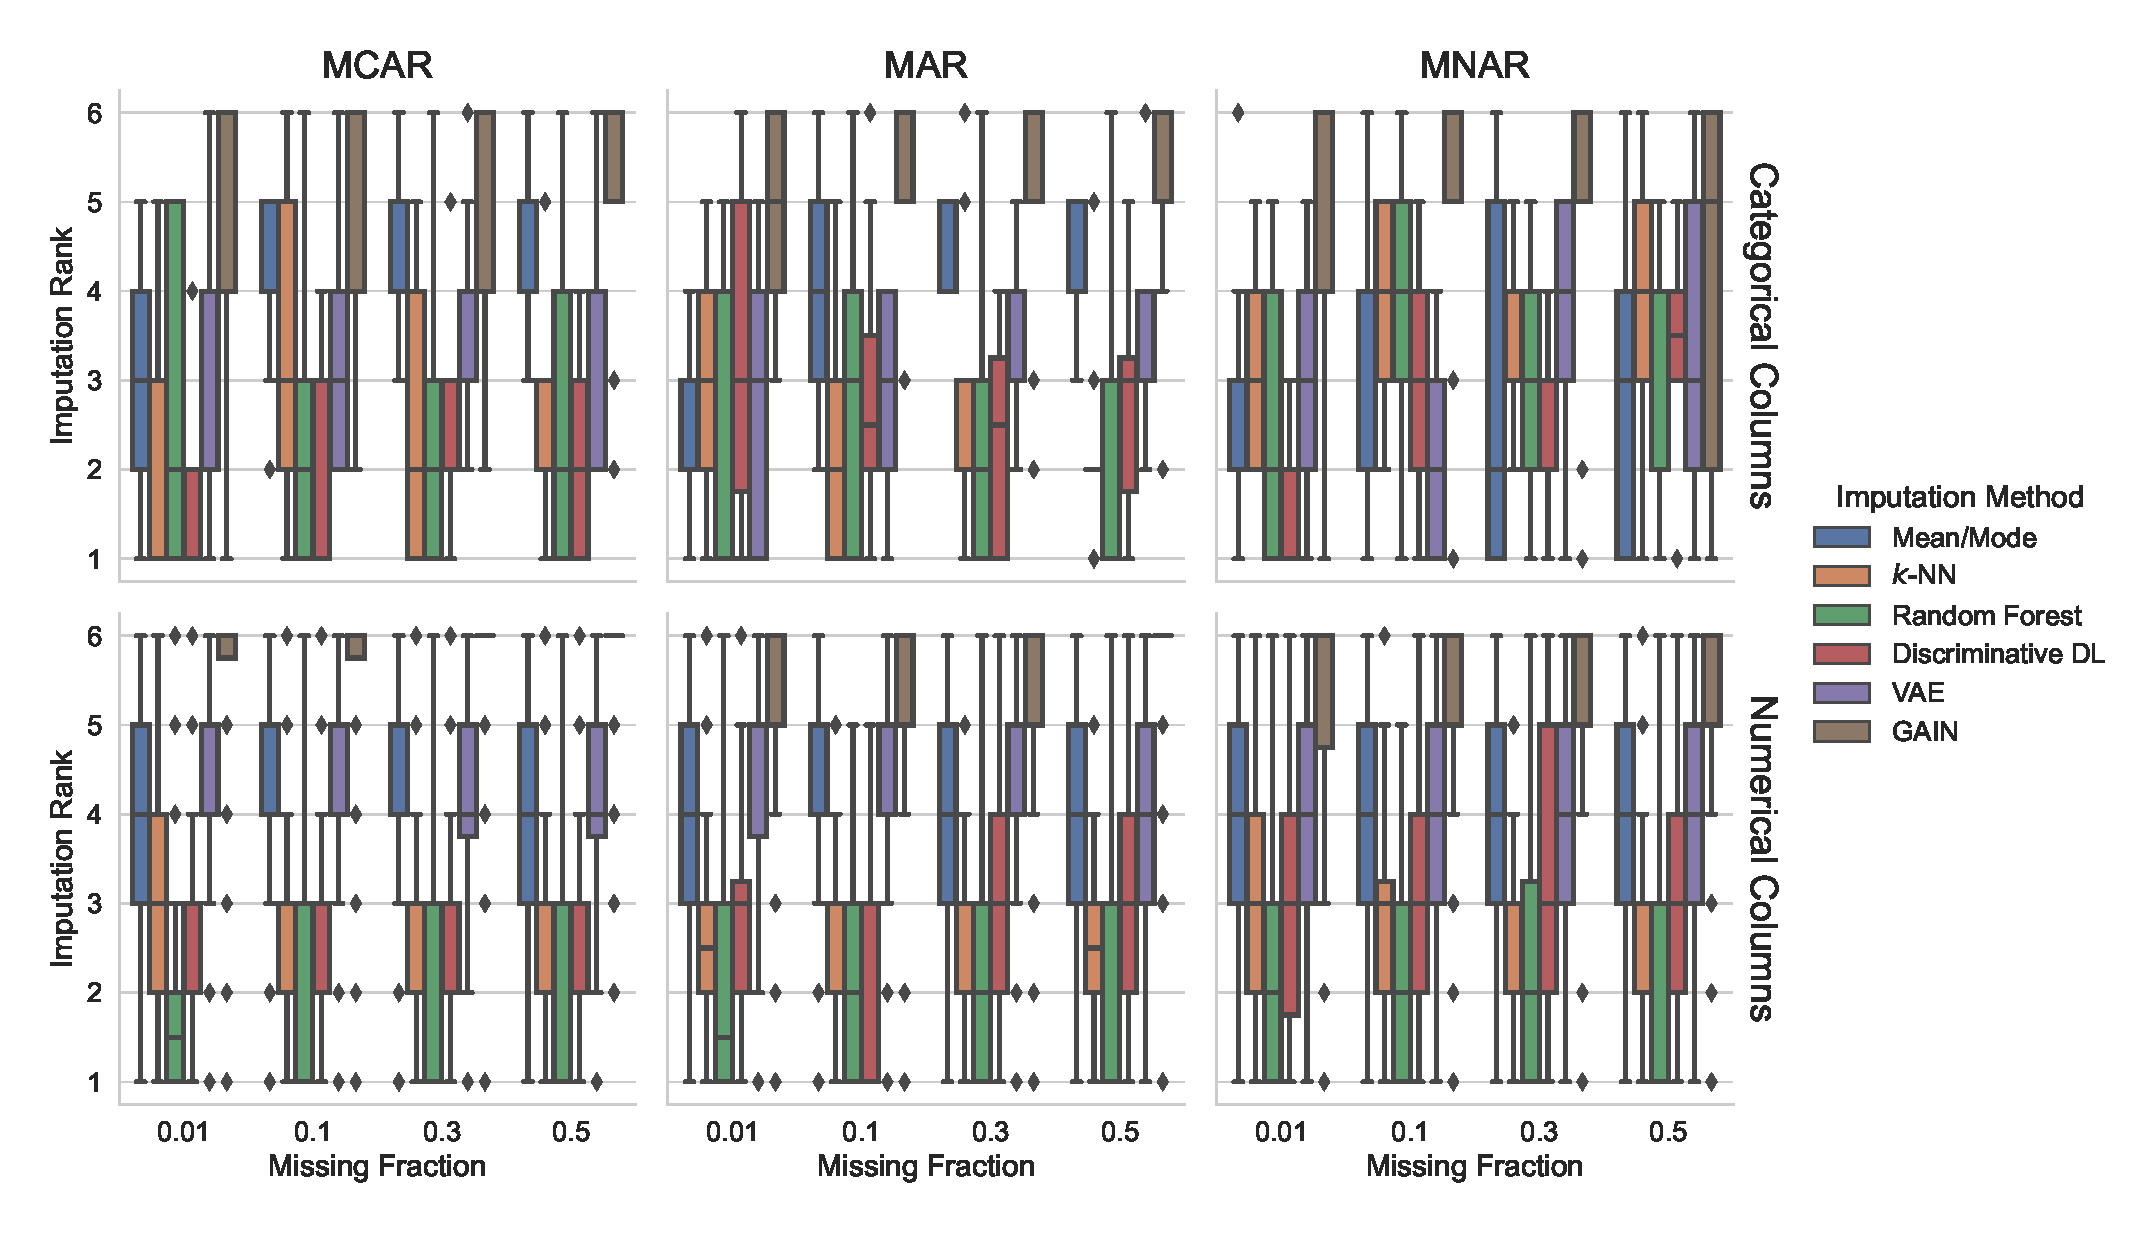
\includegraphics[width=1\columnwidth]{fully_observed_impute_rank_boxplot.eps}
    \caption[Imputation Ranks - Fully Observed]{In this figure, we visualize the results of \textit{Experiment 1} (imputation quality) in the \textit{Scenario 1} setting (training on complete data). The imputation rank is plotted against the missingness fraction. The plot is divided into six sub-plots, with three columns determined by the missingness type, ordered by task difficulty from easiest to hardest (MCAR, MAR, MNAR). In the first row of sub-plots we depict results of classification tasks, whereas the second row contains regression results. Within a single sub-plot, each box represents the distibution of ranks of a single imputer over all corresponding datasets/columns.}\label{fig:fully_observed_impute_rank_boxplot}
\end{figure}

In Figure \ref{fig:fully_observed_impute_rank_boxplot} we observe that ..
When imputing categorical columns, there is no clear winner. However, the Discriminate DL yields stronges performance in most cases. However, in the MAR setting, also the classical ML methods are among the first two to three ranks often times. With increasing complexity the DL based methods seem to improve. Interesingly though, the Mean/Mode imputation yields a lot of good results in the most complex settings.
The clear loser seems to be GAIN, with worst performance in most cases. However, in the setting of highest complexity (MNAR with 50\% missing values) the results are not as bad.

When it comes to imputing numerical columns, the picture is much clearer. Random Forest is the only method with 50\% of values among the first three ranks basically all of the time. However, the whiskers indicate that there are also some results ranging on the middle and even last ranks. \textit{k}-NN and Discriminate DL are almost as strong with the boxes indicating many second and third ranks, with k-NN performing a bit better. Mean/Mode and VAE are in the middle with the former in being slightly in the lead. Again, GAIN performs worst, this time even more clearly.

The bottom line is that the classical ML methods and discriminative DL perform best. However, for categorical columns there is often no improvement over Mode imputation. The generative methods are mostly outperformed even by Mean/Mode with VAE not as clearly as GAIN.



\subsubsection{Scenario 2: Training on Incomplete/Imputed Data}


\begin{figure}\centering
    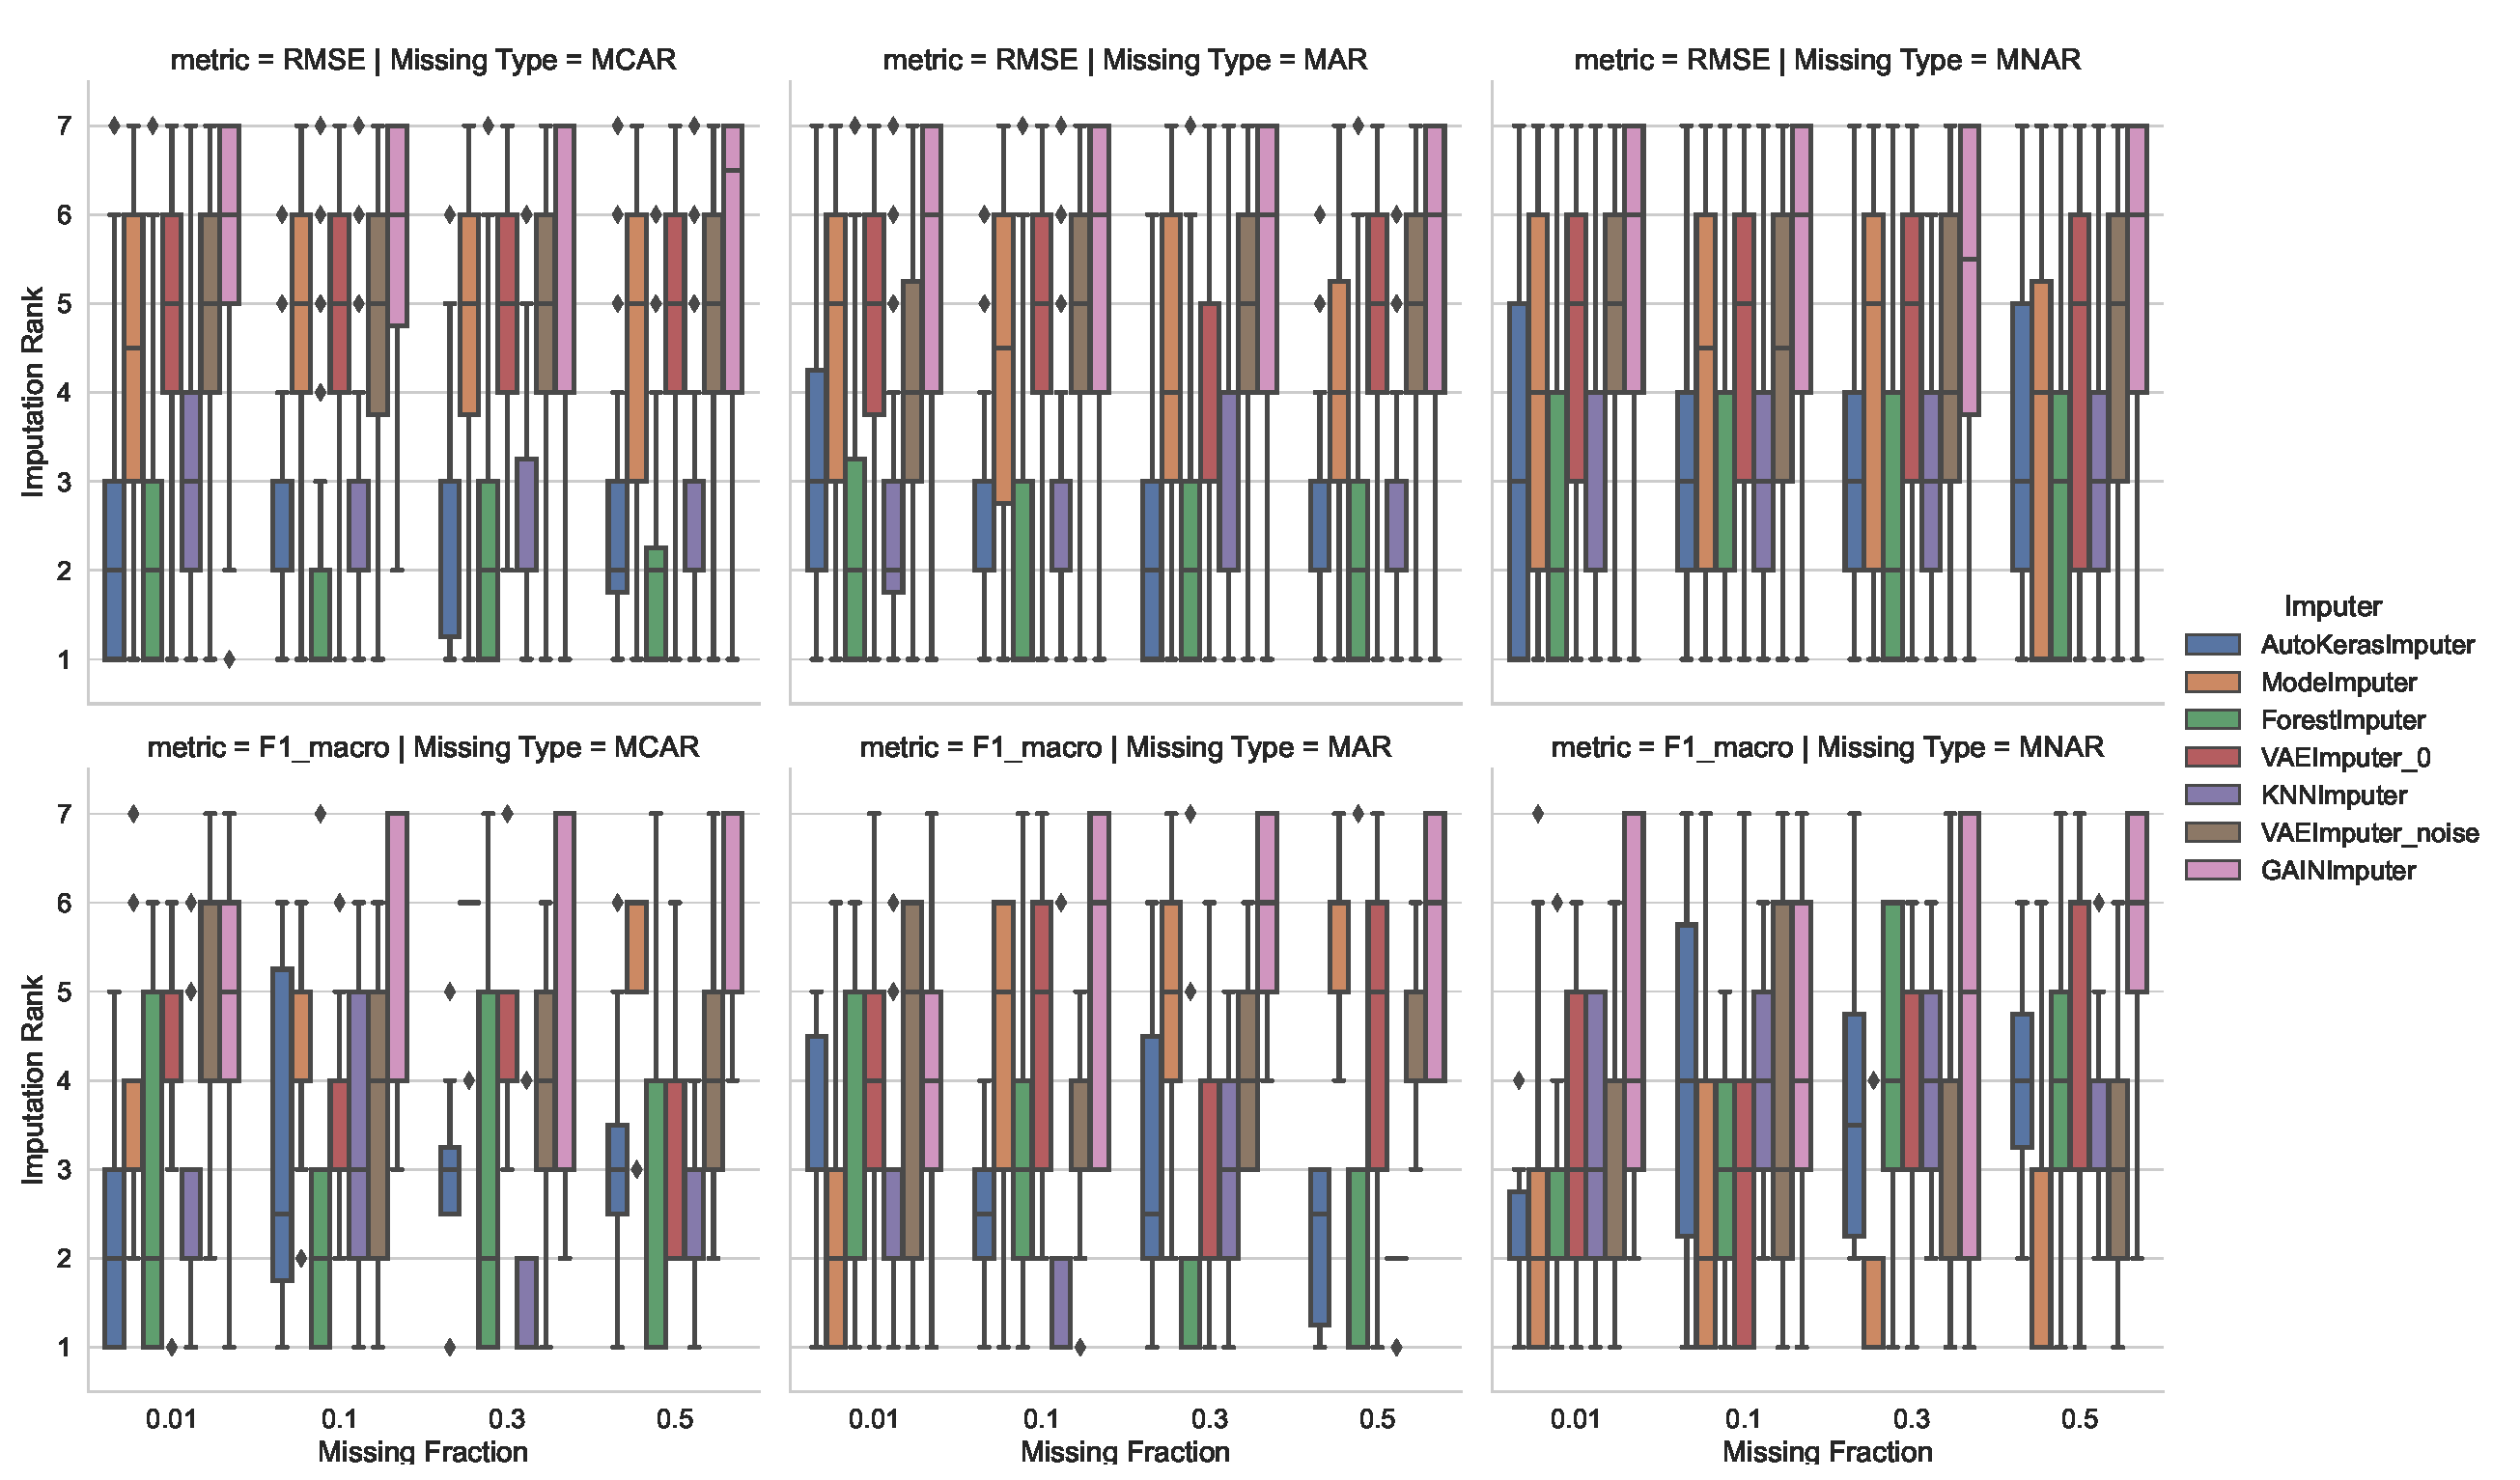
\includegraphics[width=1\columnwidth]{corrupted_impute_rank_boxplot.eps}

    \caption[Imputation Ranks - Corrupted]{In this figure, we visualize the results of \textit{Experiment 1} (imputation quality) in the \textit{Scenario 2} setting (training on incomplete/imputed data). The imputation rank is plotted against the missingness fraction. The plot is divided into six sub-plots, with three columns determined by the missingness type, ordered by task difficulty from easiest to hardest (MCAR, MAR, MNAR). In the first row of sub-plots we depict results of classification tasks, whereas the second row contains regression results. Within a single sub-plot, each box represents the distibution of ranks of a single imputer over all corresponding datasets/columns.
    }
	\label{fig:corrupted_impute_rank_boxplot}
\end{figure}

Figure \ref{fig:corrupted_impute_rank_boxplot} shows the imputation performance in \textit{Scenario 2}, i.e. when training on incomplete/imputed data. For categorical columns it is even harder to find clear patterns. With increasing task difficulty, the performance of the Mode imputation increases, though with higher variance. Interestingly, Mode outperforms other methods especially in the hardest settings (MNAR with 30\% and 50\% missing values). The classical ML methods (k-NN and Random Forest) perform pretty good on the MCAR and MAR patterns, but Random Forest has much higher variance. Discriminative DL yields similar perforamnce in these settings, slightly worse on average and with lower variance than Random Forest. For MCAR and MAR these three methods tend to yield better imputation performance than simply using Mode, especially with an increasing fraction of missing values. The generative models tend to performc worst, especially GAIN.

For numerical columns, again, the results are distinguished more clearly. The classical models yield best performances with a tendency of Random Forest to outperform k-NN, with larger variance of Random Forest however. The Discrimanative DL methods yields similar performance to the classical ML approaches in the MCAR and MAR settings. However, in the more difficult MNAR setting it performns slightly worse. In the midfield here, too, are Mean and VAE. The latter performs a slightly worse overall. On the last ranks is GAIN once again.

Overall, the results of \textit{Scenario 1} (Figure \ref{fig:fully_observed_impute_rank_boxplot}) and \textit{Scenario 2} (Figure \ref{fig:corrupted_impute_rank_boxplot}) for numeric columns are quite similar. GAIN has become somewhat better in Scenario 2, although it still ranks at the bottom. For the categorical columns, the visualizations of the two scenarios differ slightly more. However, there are no major shifts in which the median worsens by more than 2 ranks. \arndt{das habe ich nur aus den Plots abgelesen, ggf. Auswertung hierzu fahren}. Interestingly, it happens four times in scenario 2 that the complete box of MODE is on only one rank. This also occurs in KNN, once in scenario 1 and once in scenario 2.

One reason why GAIN performed so badly is it's numerical instability. Out of our 828 runs per imputer GAIN failed 273 times, that's 33\%. Besides GAIN, only the Discrimanative DL failed 3 times. \arndt{AutoKeras results where not complete yet - check again}. Thus, the last rank has been assigned to GAIN in these cases.



\subsection{Experiment 2: Impact on Downstream Task}


\subsubsection{Scenario 1: Training on Complete Data}


\begin{figure}\centering
	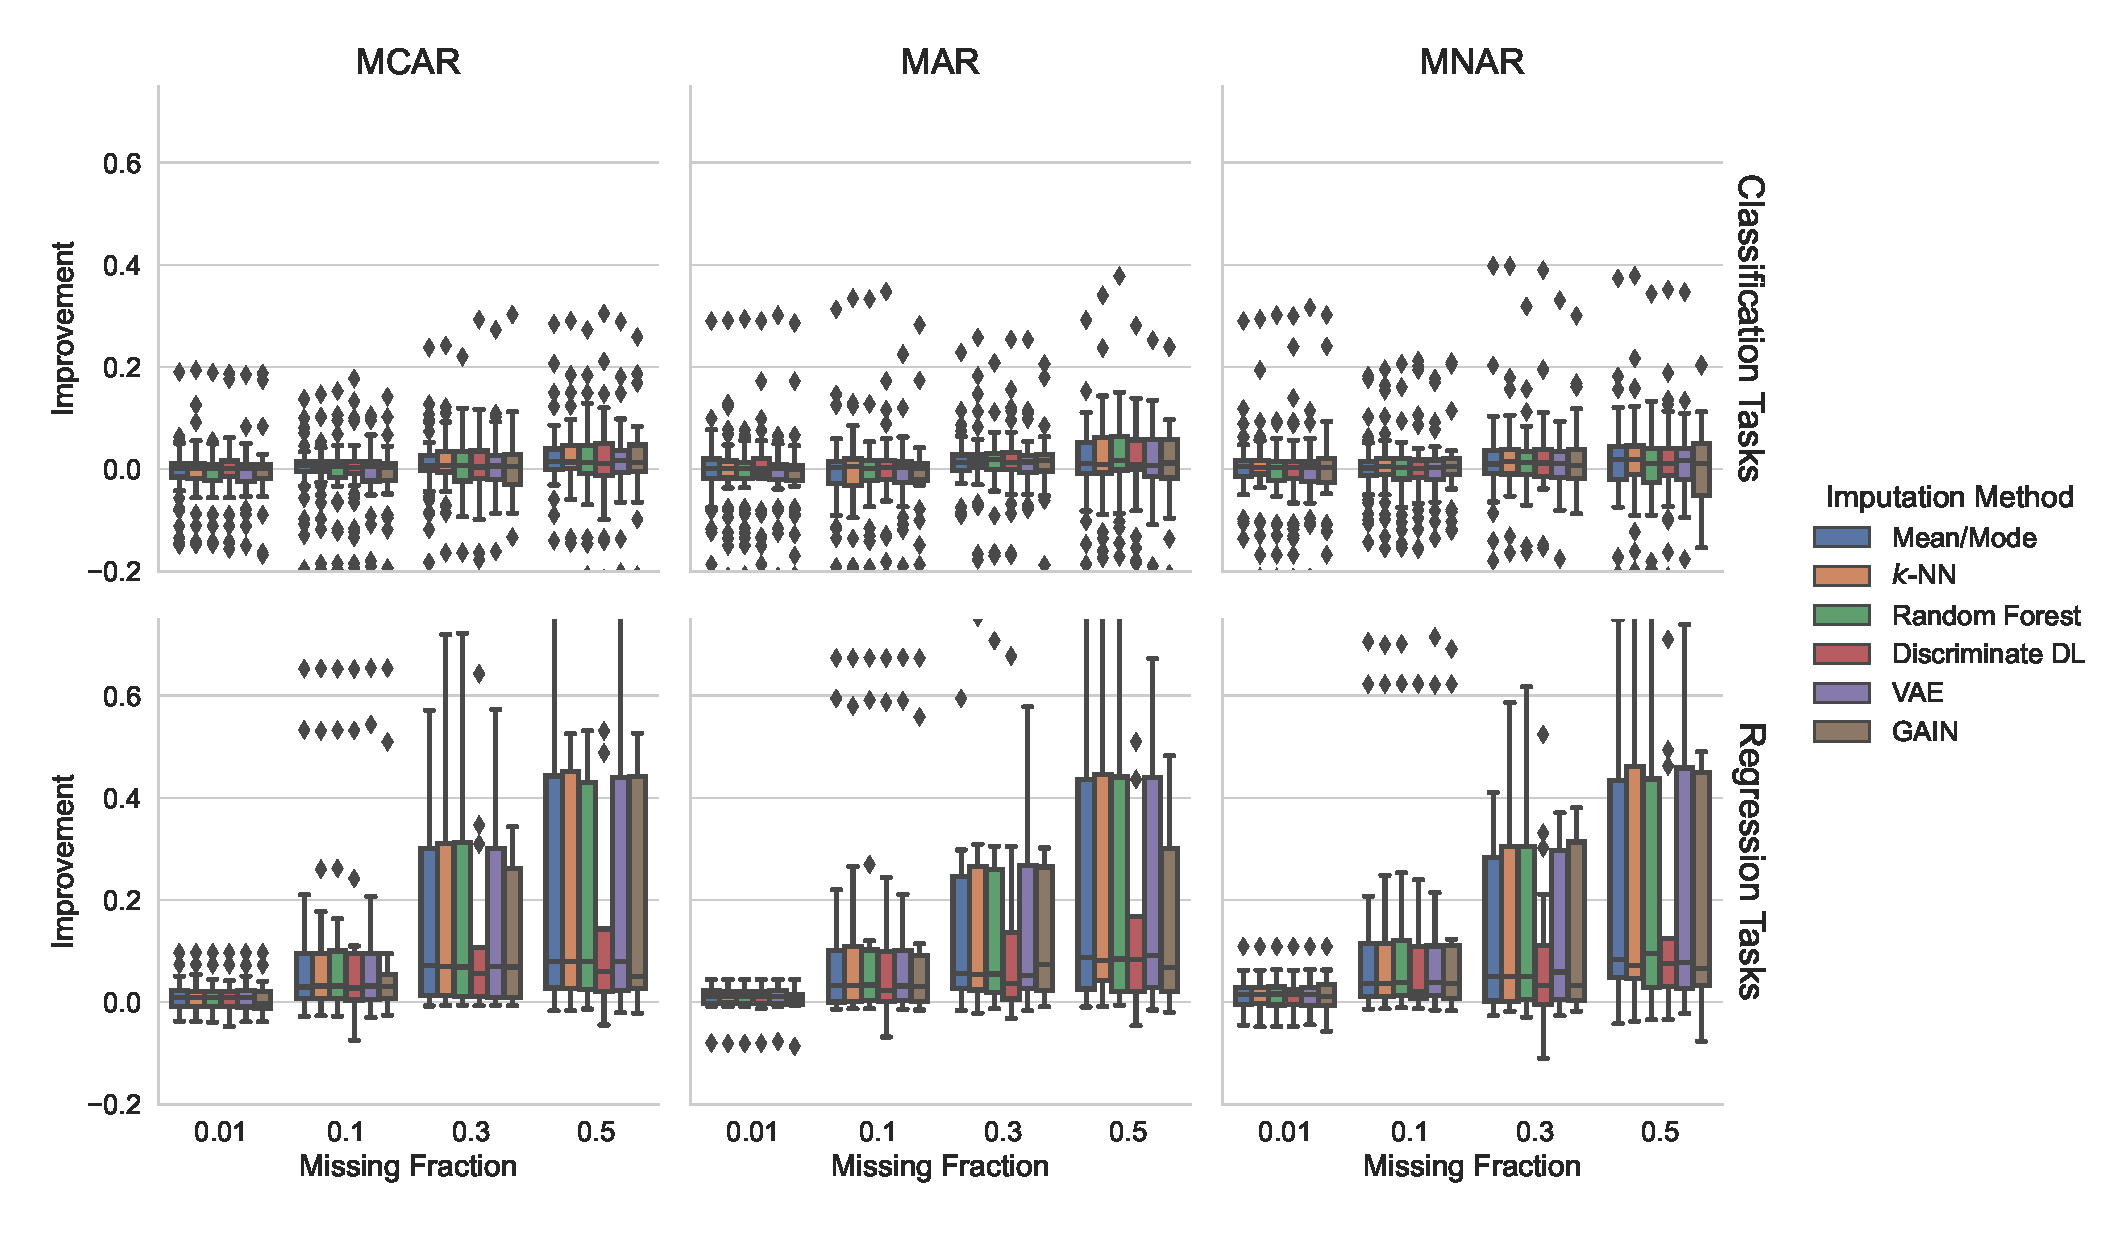
\includegraphics[width=1\columnwidth]{fully_observed_downstream_boxplot.eps}

	\caption[Downstream Ranks - Fully Observed]{In this figure, we visualize the results of \textit{Experiment 2} (impact on downstream task) in the \textit{Scenario 1} setting (training on complete data). The downstream rank is plotted against the missingness fraction. The plot is divided into six sub-plots, with three columns determined by the missingness type, ordered by task difficulty from easiest to hardest (MCAR, MAR, MNAR). In the first row of sub-plots we depict results of classification tasks, whereas the second row contains regression results. Within a single sub-plot, each box represents the distibution of ranks of a single imputer over all corresponding datasets/columns.
    }
	\label{fig:fully_observed_downstream_boxplot}
\end{figure}

TODO XXXXX


\subsubsection{Scenario 2: Training on Incomplete/Imputed Data}


\begin{figure}\centering
	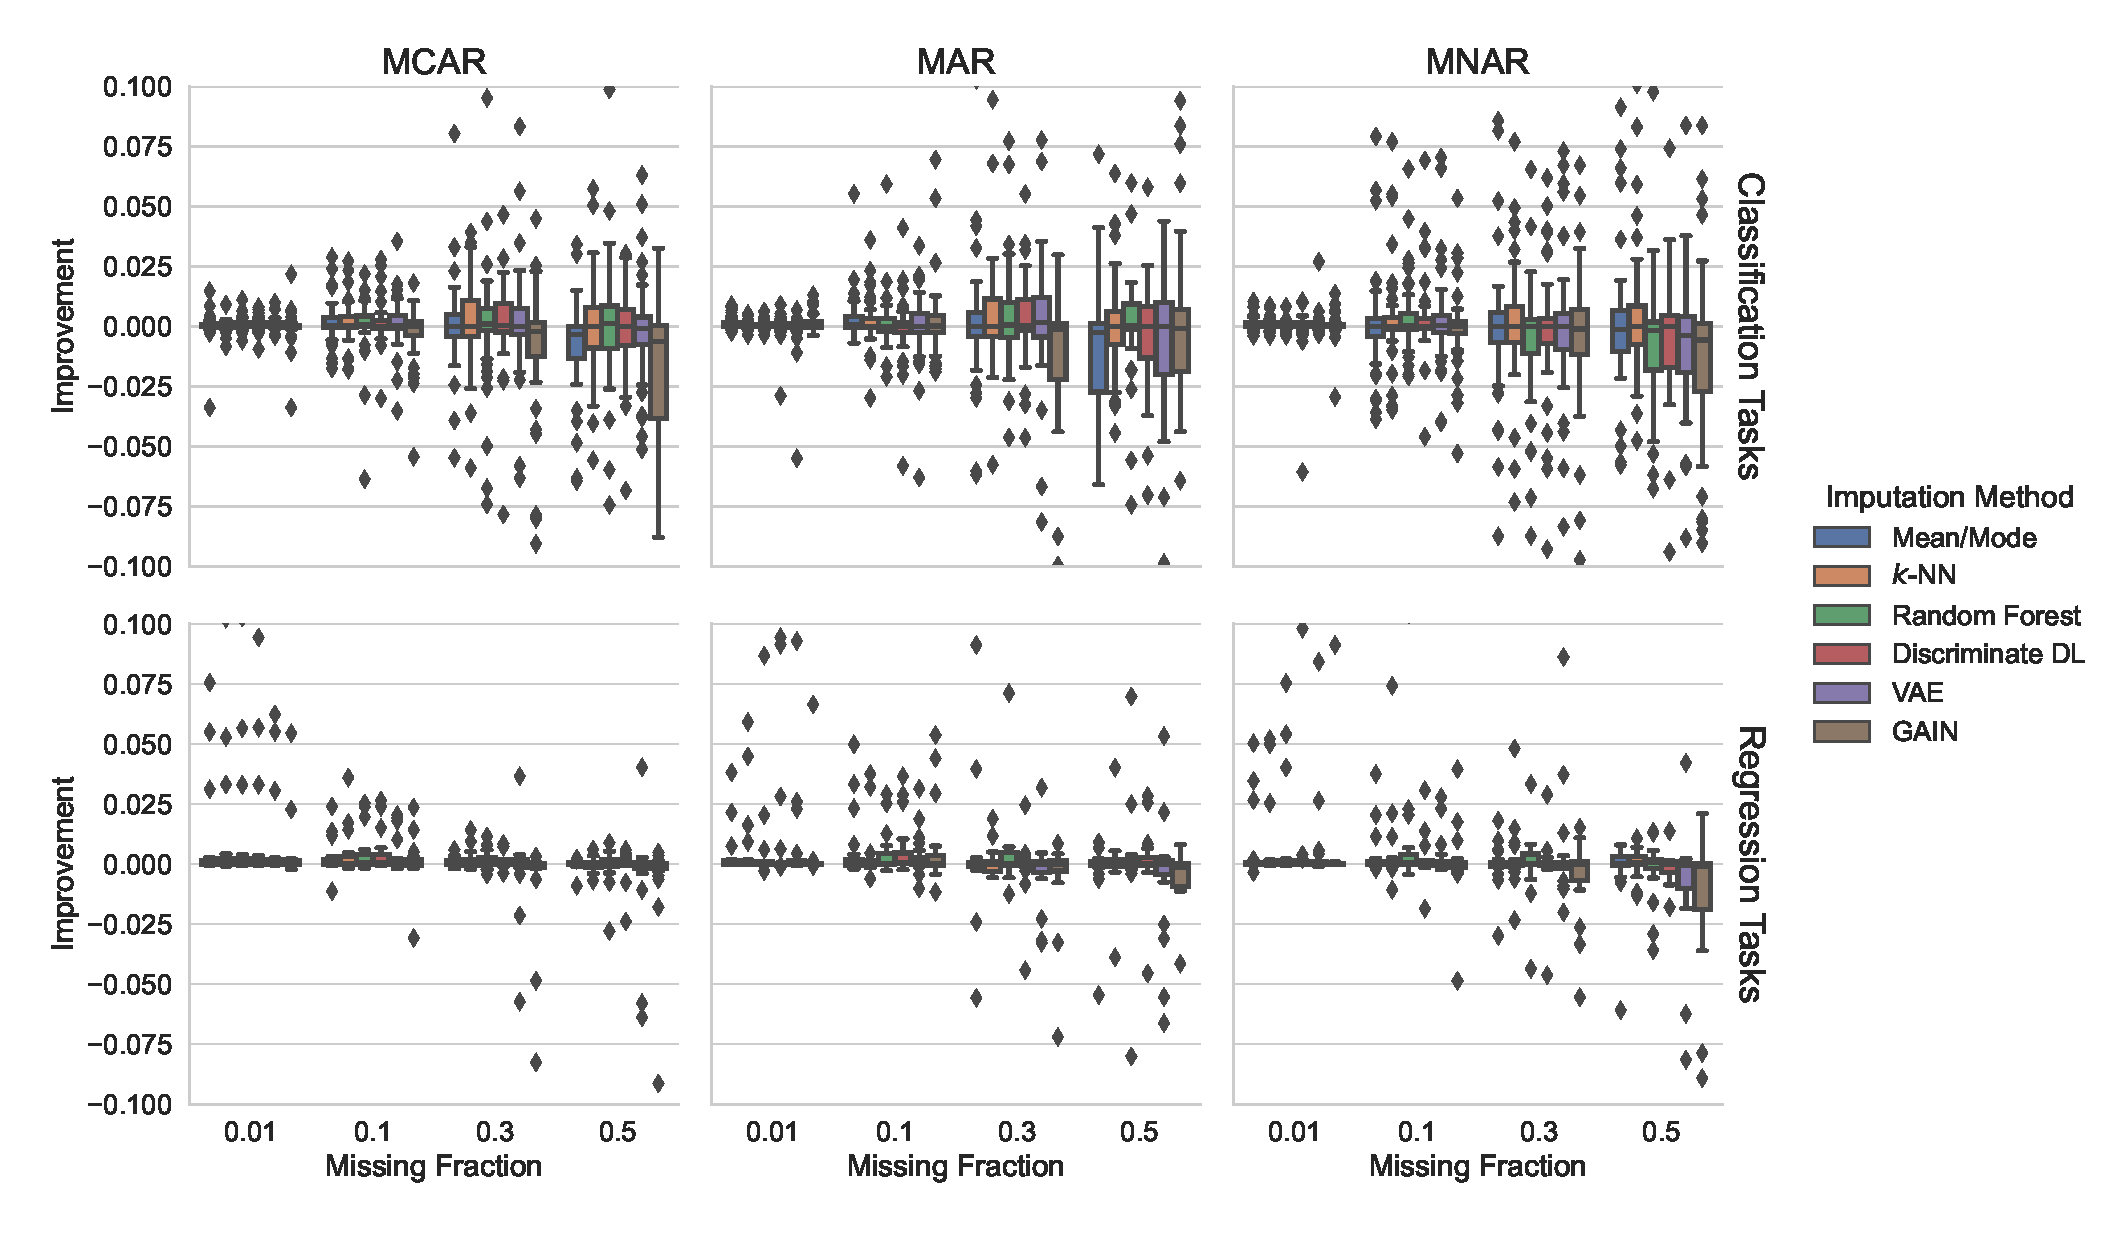
\includegraphics[width=1\columnwidth]{corrupted_downstream_boxplot.eps}

	\caption[Downstream Ranks - Corrupted]{In this figure, we visualize the results of \textit{Experiment 2} (impact on downstream task) in the \textit{Scenario 2} setting (training on incomplete/imputed data). The downstream rank is plotted against the missingness fraction. The plot is divided into six sub-plots, with three columns determined by the missingness type, ordered by task difficulty from easiest to hardest (MCAR, MAR, MNAR). In the first row of sub-plots we depict results of classification tasks, whereas the second row contains regression results. Within a single sub-plot, each box represents the distibution of ranks of a single imputer over all corresponding datasets/columns.
    }
	\label{fig:corrupted_downstream_boxplot}
\end{figure}

TODO XXXXX



Conclusions:
- higher variance of random forest over knn due to outliers ?!
- generative methods mostly worse than mean/mode
- discriminative often as good as classical ML and better than mean/mode, but when considering
the runtime might not be a good choice
